\chapter{Unfolding}
\label{app:Unfolding}

For any experiment, there is a disconnect between the desired phenomena (\emph{truth} level) and the measurement (\emph{measured} level) due to limitations of the detector setup. This is portrayed in Fig.~\ref{fig:UnfoldingScheme} through a dijet event at the truth level, whose final state charged and neutral particles are recorded as TPC tracks and BEMC towers.  Each of the detectors smear the energy and momenta and for almost all experiments,  the information about particle species is lost. For example, at STAR often a \(\pi^0\) mass assumption is taken for measured constituents. Thus jets, which are composite objects of these tracks and towers are non-trivially modified by a complicated convolution of these effects. Even with the best background removal procedure, jets will contain some residual background fluctuations from the underlying event.

\begin{figure}
	\centering
	\begin{tikzpicture}[scale=0.7,rotate=0]
		\def\R{5} % tracker outer radius
		\def\dang{3} % angular granularity of calo deposits, 
		% HCAL DEPOSITS
		\foreach \dr [count=\i,
		evaluate={\r=\R+\dr; \anga=12+\dang*\i; \angb=\anga+\dang;}
		] in {0.1, 0.2, 0.2, 0.6, 0.3,0.5,0.2,2.0,1.2,0.3,0.5, 0.2, 0.4, 0.1}{
			\draw[calo] (0,0) -- (\anga:\r) arc(\anga:\angb:\r) -- cycle;
			%\draw[calo]
			%  (\anga:\R) -- (\anga:\r) arc(\anga:\angb:\r)
			%  -- (\angb:\R) arc(\angb:\anga:\R) -- cycle;
		}
		
		\foreach \dr [count=\i,
		evaluate={\r=\R+\dr; \anga=192+\dang*\i; \angb=\anga+\dang;}
		] in {0.1, 0.05, 0.3, 0.2,0.3,0.5,0.2, 0.5,0.4,0.3,0.5, 0.2, 0.4, 0.1}{
			\draw[calo] (0,0) -- (\anga:\r) arc(\anga:\angb:\r) -- cycle;
			%\draw[calo]
			%  (\anga:\R) -- (\anga:\r) arc(\anga:\angb:\r)
			%  -- (\angb:\R) arc(\angb:\anga:\R) -- cycle;
		}
		
		\foreach \ang [count=\i, 
		evaluate={\stepa = 15;
			\stepb=\stepa+50;
			\ra=\R+0.25*sin(\dang*\i*10); 
			\rb=\R+0.2*cos(\dang*\i*15);
			\rc=\R+0.3*sin(\dang*\i*20);
			\rd=\R+0.1;
		}]in {0, 3,...,360}{
			\draw[calobg] (0,0) -- (\ang:\ra) arc(\ang:\ang+\dang:\ra) -- cycle;
			\draw[calobg] (0,0) -- (\ang:\rd) arc(\ang:\ang+\dang:\rd) -- cycle;
			\draw[calobg] (0,0) -- (\stepa*\dang+\ang:\rb) arc(\stepa*\dang+\ang:\stepa*\dang+\ang+\dang:\rb) -- cycle;
			\draw[calobg] (0,0) -- (\stepb*\dang+\ang:\rc) arc(\stepb*\dang+\ang:\stepb*\dang+\ang+\dang:\rc) -- cycle;
		}
		
		\draw[thick,fill=white] (0,0) circle(\R); 
		
		\foreach \ang [count=\i,
		evaluate={\bend=12*sin(20+\i*\dang*15)}]in {0, 3,...,360}{
			\draw[black,opacity=0.3,thin,fill=none]
			(0,0) to[bend right=\bend] (\ang:\R);
		}
		
		\foreach \ang [count=\i,
		evaluate={\bend=12*cos(\i*\dang*15)}]in {0, 3,...,360}{
			\draw[black,opacity=0.3,thin,fill=none]
			(0,0) to[bend left=\bend] (\ang-\dang*0.5:\R);
		}
		
		%\draw[calo]
		%  (\anga:\R) -- (\anga:\r) arc(\anga:\angb:\r)
		%  -- (\angb:\R) arc(\angb:\anga:\R) -- cycle;
		
		\foreach \bend [count=\i,
		evaluate={\anga=6+\dang*\i;}
		] in {30, 14, 15,18, 20, 12, 19, 17, 11, 12}{
			\draw[blue!60!green!50!black,thin,fill=none]
			(0,0) to[bend left=\bend] (\anga:\R);	
		}	
		
		\foreach \bend [count=\i,
		evaluate={\anga=72-\dang*\i;}
		] in {20, 30, 19, 18, 20, 12, 19, 17, 12, 10, 8}{
			\draw[blue!60!green!50!black,thin,fill=none]
			(0,0) to[bend right=\bend] (\anga:\R);
		}
		
		\foreach \bend [count=\i,
		evaluate={\anga=186+1.5*\dang*\i;}
		] in {30, 14, 20, 12, 11, 12}{
			\draw[blue!60!green!50!black,thin,fill=none]
			(0,0) to[bend left=\bend] (\anga:\R);
		}
		
		\foreach \bend [count=\i,
		evaluate={\anga=252-1.5*\dang*\i;}
		] in {20, 30, 19, 12, 19, 10, 8}{
			\draw[blue!60!green!50!black,thin,fill=none]
			(0,0) to[bend right=\bend] (\anga:\R);
		}
		
		\node[draw, text width=0.15\textwidth, rounded corners=4pt] (tracks) at (90:1.3*\R){
			\textbf{TPC tracks}
		};		
		\draw (tracks) edge[dashed,  ->, very thick, red] (225:0.6*\R);
		\draw (tracks) edge[dashed,  ->, very thick, red] (30:0.5*\R);
		
		\node[draw, text width=0.17\textwidth, rounded corners=4pt] (towers) at (150:1.5*\R){
			\textbf{BEMC tower deposits} 
		};		
		\draw (towers) edge[dashed,  ->, very thick, magenta] (210:1.02*\R);
		\draw (towers) edge[dashed,  ->, very thick, magenta] (30:1.02*\R);
		
		\node[draw, text width=0.15\textwidth, rounded corners=4pt] (UE) at (340:1.8*\R){
			\textbf{Underlying Event}
		};		
		\draw (UE) edge[dashed, ->, very thick, blue] (300:1.02*\R);
		\draw (UE) edge[dashed,  ->, very thick, blue] (340:0.5*\R);
		
		\draw[thick,fill=white] (0,0) circle(0.27*\R); 
		\begin{feynhand}[scale=0.3]
			\vertex (a)  at (-1, -2); 
			\vertex(b)  at (-2, 1); 
			\vertex (c)  at (0, -1); 
			\vertex (d)  at (0, 1);
			\propag [plain] (c) to (a);
			\propag [plain] (b) to  [edge label = $p_1$] (d);
			\propag [gluon] (c) to (d);
			\vertex(e) at (2, -1) ; 
			\vertex (f) at (1, 2);
			\propag [plain] (e) to [edge label = $p_2$](c);
			\propag [plain] (d) to (f);
			\coordinate (J1) at (2.5,3.5);
			\coordinate (J2) at (-2.5, -3.5);
			\jetcone{f}{J1}{0.4}{0.10}
			\jetcone{a}{J2}{0.4}{0.10}
			\node[vector,left] at (J1) {$\vv{p}_{j_1}$};
			\node[vector,right] at (J2) {$\vv{p}_{j_2}$};
		\end{feynhand}		
		
		\draw  (10:\R) edge["\textbf{Deconvolution / Unfolding}", ->, very thick, red] (10:0.15*\R);
	\end{tikzpicture}
	\caption[Schematic of the unfolding of detector effects]{Schematic figure showing the unfolding procedure. The desired physics / truth / particle level is represented by the \(2\to 2\) Feynman diagram in the middle. The blue (gray) tracks and tower deposits are the dijet (underlying) event as recorded by the TPC and BEMC. }
	\label{fig:UnfoldingScheme} 
\end{figure}

Thus distributions of any jet observable \(\mathbf{O}\) will have these \emph{detector effects} which will need to be removed in order for the measurement to be comparable to theory calculations. In other terms, a truth value of \(\mathbf{x}\) can manifest as a range of measured values \((\mathbf{x}_0, \mathbf{x}_1)\) similarly, a measured value of \(\mathbf{y}\) can come from a range of truth values \((\mathbf{y}_0, \mathbf{y}_1)\).  Thus, using Bayes theorem, the probability either measured value being  \(\mathbf{y}\)  or truth value being  \(\mathbf{x}\) would be,

\begin{align}
	\label{eq:trMeas}
	p_\mathrm{meas.}(\mathbf{y}) &= \int d\mathbf{x}~p_\mathrm{meas.|tr.}(\mathbf{y} |  \mathbf{x}) p_\mathrm{tr.}(\mathbf{x}) \notag\\
	p_\mathrm{tr.}(\mathbf{x}) &= \int d\mathbf{y}~p_\mathrm{tr.|meas.}(\mathbf{x} |  \mathbf{y}) p_\mathrm{meas.}(\mathbf{y}).
\end{align}



From Eq.~\ref{eq:trMeas}, we measure \(p_\mathrm{meas.}\) through histograms, density estimates, etc. and \(p_\mathrm{tr.}\) is what we want to determine. Now, \(p_\mathrm{meas.|tr.}\) represents the detector's \emph{response}, which can be obtained to a high degree of accuracy from simulation programs like GEANT~\cite{MISC-15}. We can start from a \emph{generated} truth distribution  \(p_\mathrm{gen., 0}\) and obtain the \emph{reconstructed} measured distribution  \(p_\mathrm{reco., 0}\). Thus the assumption is, 
\begin{align}
	\label{eq:responseTransfer}
	p_\mathrm{meas.|tr.}(\mathbf{y} |  \mathbf{x}) = p_\mathrm{reco.|gen., 0}(\mathbf{y} |  \mathbf{x}) \equiv R(\mathbf{y}, \mathbf{x}) ,
\end{align}
Substituting \(R(\mathbf{y}, \mathbf{x})\) in Eq.~\ref{eq:trMeas} and using \(\omega_0(\mathbf{y}) = p_\mathrm{meas.}(\mathbf{y})/p_\mathrm{reco., 0}(\mathbf{y})\)
\begin{align}
	\label{eq:unfoldEstimator}
	p_\mathrm{gen., 1}(\mathbf{x}) &\equiv \int d\mathbf{y}~p_\mathrm{gen.|reco., 0}(\mathbf{x} |  \mathbf{y})\,p_\mathrm{meas.}(\mathbf{y}) \notag\\
	&=\int d\mathbf{y}~\frac{R(\mathbf{y}, \mathbf{x})\,p_\mathrm{gen., 0}(\mathbf{x})}{p_\mathrm{reco., 0}(\mathbf{y})} p_\mathrm{meas.}(\mathbf{y})\notag\\
	&= p_\mathrm{gen., 0}(\mathbf{x})\int d\mathbf{y}~R(\mathbf{y}, \mathbf{x})\,\omega_0(\mathbf{y}).
\end{align}
Using \(\nu_0(\mathbf{x}) = p_\mathrm{gen., 1}(\mathbf{x})/p_\mathrm{gen., 0}(\mathbf{x})\) measured distribution correspondingly becomes,
\begin{align}
	\label{eq:step2Joint}
	p_\mathrm{reco., 1}(\mathbf{y}) &= \int d\mathbf{x}~(\mathbf{x})\,R(\mathbf{y}, \mathbf{x})\,p_\mathrm{gen., 1}(\mathbf{x})\notag\\
	&= p_\mathrm{reco., 0}(\mathbf{y}) \int d\mathbf{x}~\frac{R(\mathbf{y}, \mathbf{x})\,p_\mathrm{gen., 0}(\mathbf{x})}{p_\mathrm{reco., 0}(\mathbf{y})}\nu_0(\mathbf{x}). 
\end{align}
The convolutions \(\int d\mathbf{y}~R(\mathbf{y}, \mathbf{x})\,\omega_0(\mathbf{y})\) and \(\int d\mathbf{x}~R(\mathbf{y}, \mathbf{x})\frac{\,p_\mathrm{gen., 0}(\mathbf{x})}{p_\mathrm{reco., 0}(\mathbf{y})}\nu_0(\mathbf{x})\) are mapping \(\omega_0(\mathbf{y})\to\omega_0(\mathbf{x})\) and \(\nu_0(\mathbf{x})\to\nu_0(\mathbf{y})\) respectively. 
%
For the \(n^\text{th}\) iteration, 
%
\begin{align}
	\label{eq:generalUnfolding}
	\omega_{n-1}(\mathbf{y}) &= \frac{p_\mathrm{meas.}(\mathbf{y})}{p_{\mathrm{reco.}, n-1}(\mathbf{y})} \notag\\
	p_{\mathrm{gen.}, n}(\mathbf{x}) &= p_{\mathrm{gen.}, n-1}(\mathbf{x})\int d\mathbf{y}~R(\mathbf{y}, \mathbf{x})\,\omega_{n-1}(\mathbf{y})\notag\\
	\nu_{n-1}(\mathbf{x}) &= \frac{p_{\mathrm{gen.}, n}(\mathbf{x})}{p_{\mathrm{gen.}, n-1}(\mathbf{x})} \notag\\
	p_{\mathrm{reco.}, n}(\mathbf{y}) &= p_{\mathrm{reco.}, n-1}(\mathbf{y}) \int d\mathbf{x}~R(\mathbf{y}, \mathbf{x})\frac{p_{\mathrm{gen.}, n-1}(\mathbf{x})}{p_{\mathrm{reco.}, n-1}(\mathbf{y})}\nu_{n-1}(\mathbf{x}). 
\end{align}
%
Given convergence, \(p_{\mathrm{reco.}, n}(\mathbf{y}) \to p_\mathrm{gen.}(\mathbf{y})\) and \(p_{\mathrm{tr.}, n}(\mathbf{x}) \to p_{\mathrm{unf.}}(\mathbf{x})\) is the unfolded distribution. 

%Generated jets without a reconstructed partner (\emph{misses}, \(\mathbf{y}=\varnothing\)) carry no \(\omega_{n-1}\), and reconstructed jets without a generated partner (\emph{fakes}, \(\mathbf{x}=\varnothing\)) carry no \(\nu_{n-1}\). Each receives its missing weight from the corresponding map of Eq.~\ref{eq:generalUnfolding}, built from matched pairs and normalized over them,
%\begin{align}
%	\label{eq:missFakeWeights}
%	\omega_{n-1}(\mathbf{x}) &= \frac{\int d\mathbf{y}~R(\mathbf{y}, \mathbf{x})\,\omega_{n-1}(\mathbf{y})}{\int d\mathbf{y}~R(\mathbf{y}, \mathbf{x})}
%	= \frac{\int d\mathbf{y}~R(\mathbf{y}, \mathbf{x})\,\omega_{n-1}(\mathbf{y})}{\epsilon(\mathbf{x})} ,
%	&&\mathbf{y}=\varnothing , \notag\\
%	\nu_{n-1}(\mathbf{y}) &= \frac{\int d\mathbf{x}~R(\mathbf{y}, \mathbf{x})\,p_{\mathrm{gen.}, n-1}(\mathbf{x})\,\nu_{n-1}(\mathbf{x})}{\int d\mathbf{x}~R(\mathbf{y}, \mathbf{x})\,p_{\mathrm{gen.}, n-1}(\mathbf{x})} ,
%	&&\mathbf{x}=\varnothing ,
%\end{align}
%where \(\epsilon(\mathbf{x})\) is the reconstruction efficiency and the second denominator is \(p_{\mathrm{reco.}, n-1}(\mathbf{y})\) of matched jets. A miss at \(\mathbf{x}\) thus enters the second step with the mean first-step weight of the matched generated jets at \(\mathbf{x}\), and a fake at \(\mathbf{y}\) enters the next iteration with the weight the matched reconstructed jets at \(\mathbf{y}\) acquire from \(\nu_{n-1}\). Eq.~\ref{eq:generalUnfolding} then holds on the full samples,
%\begin{align}
%	\label{eq:missFakeIteration}
%	p_{\mathrm{gen.}, n}(\mathbf{x}) &= \omega_{n-1}(\mathbf{x})\,p_{\mathrm{gen.}, n-1}(\mathbf{x}) = \nu_{n-1}(\mathbf{x})\,p_{\mathrm{gen.}, n-1}(\mathbf{x}) , &&\text{matched and missed,} \notag\\
%	p_{\mathrm{reco.}, n}(\mathbf{y}) &= \nu_{n-1}(\mathbf{y})\,p_{\mathrm{reco.}, n-1}(\mathbf{y}) , &&\text{matched and fake,}
%\end{align}
%so that \(\nu_{n-1}\) is formed over a generated distribution that includes misses, and \(\omega_n\) against a reconstructed distribution that includes fakes.

This algorithm can be adapted for binned data by expressing the distributions as vectors representing bin counts of histograms and \(R(\mathbf{y}, \mathbf{x})\) as a matrix, giving the traditional method of \emph{Iterative Bayesian Unfolding}~\cite{bennerRoounfold}. Although it has been the standard for a long time, the required binning of data limits its usefulness beyond 3-dimensions. Also, not all measurements can be straightforwardly represented in the response matrix. 

\begin{figure}
	\centering
	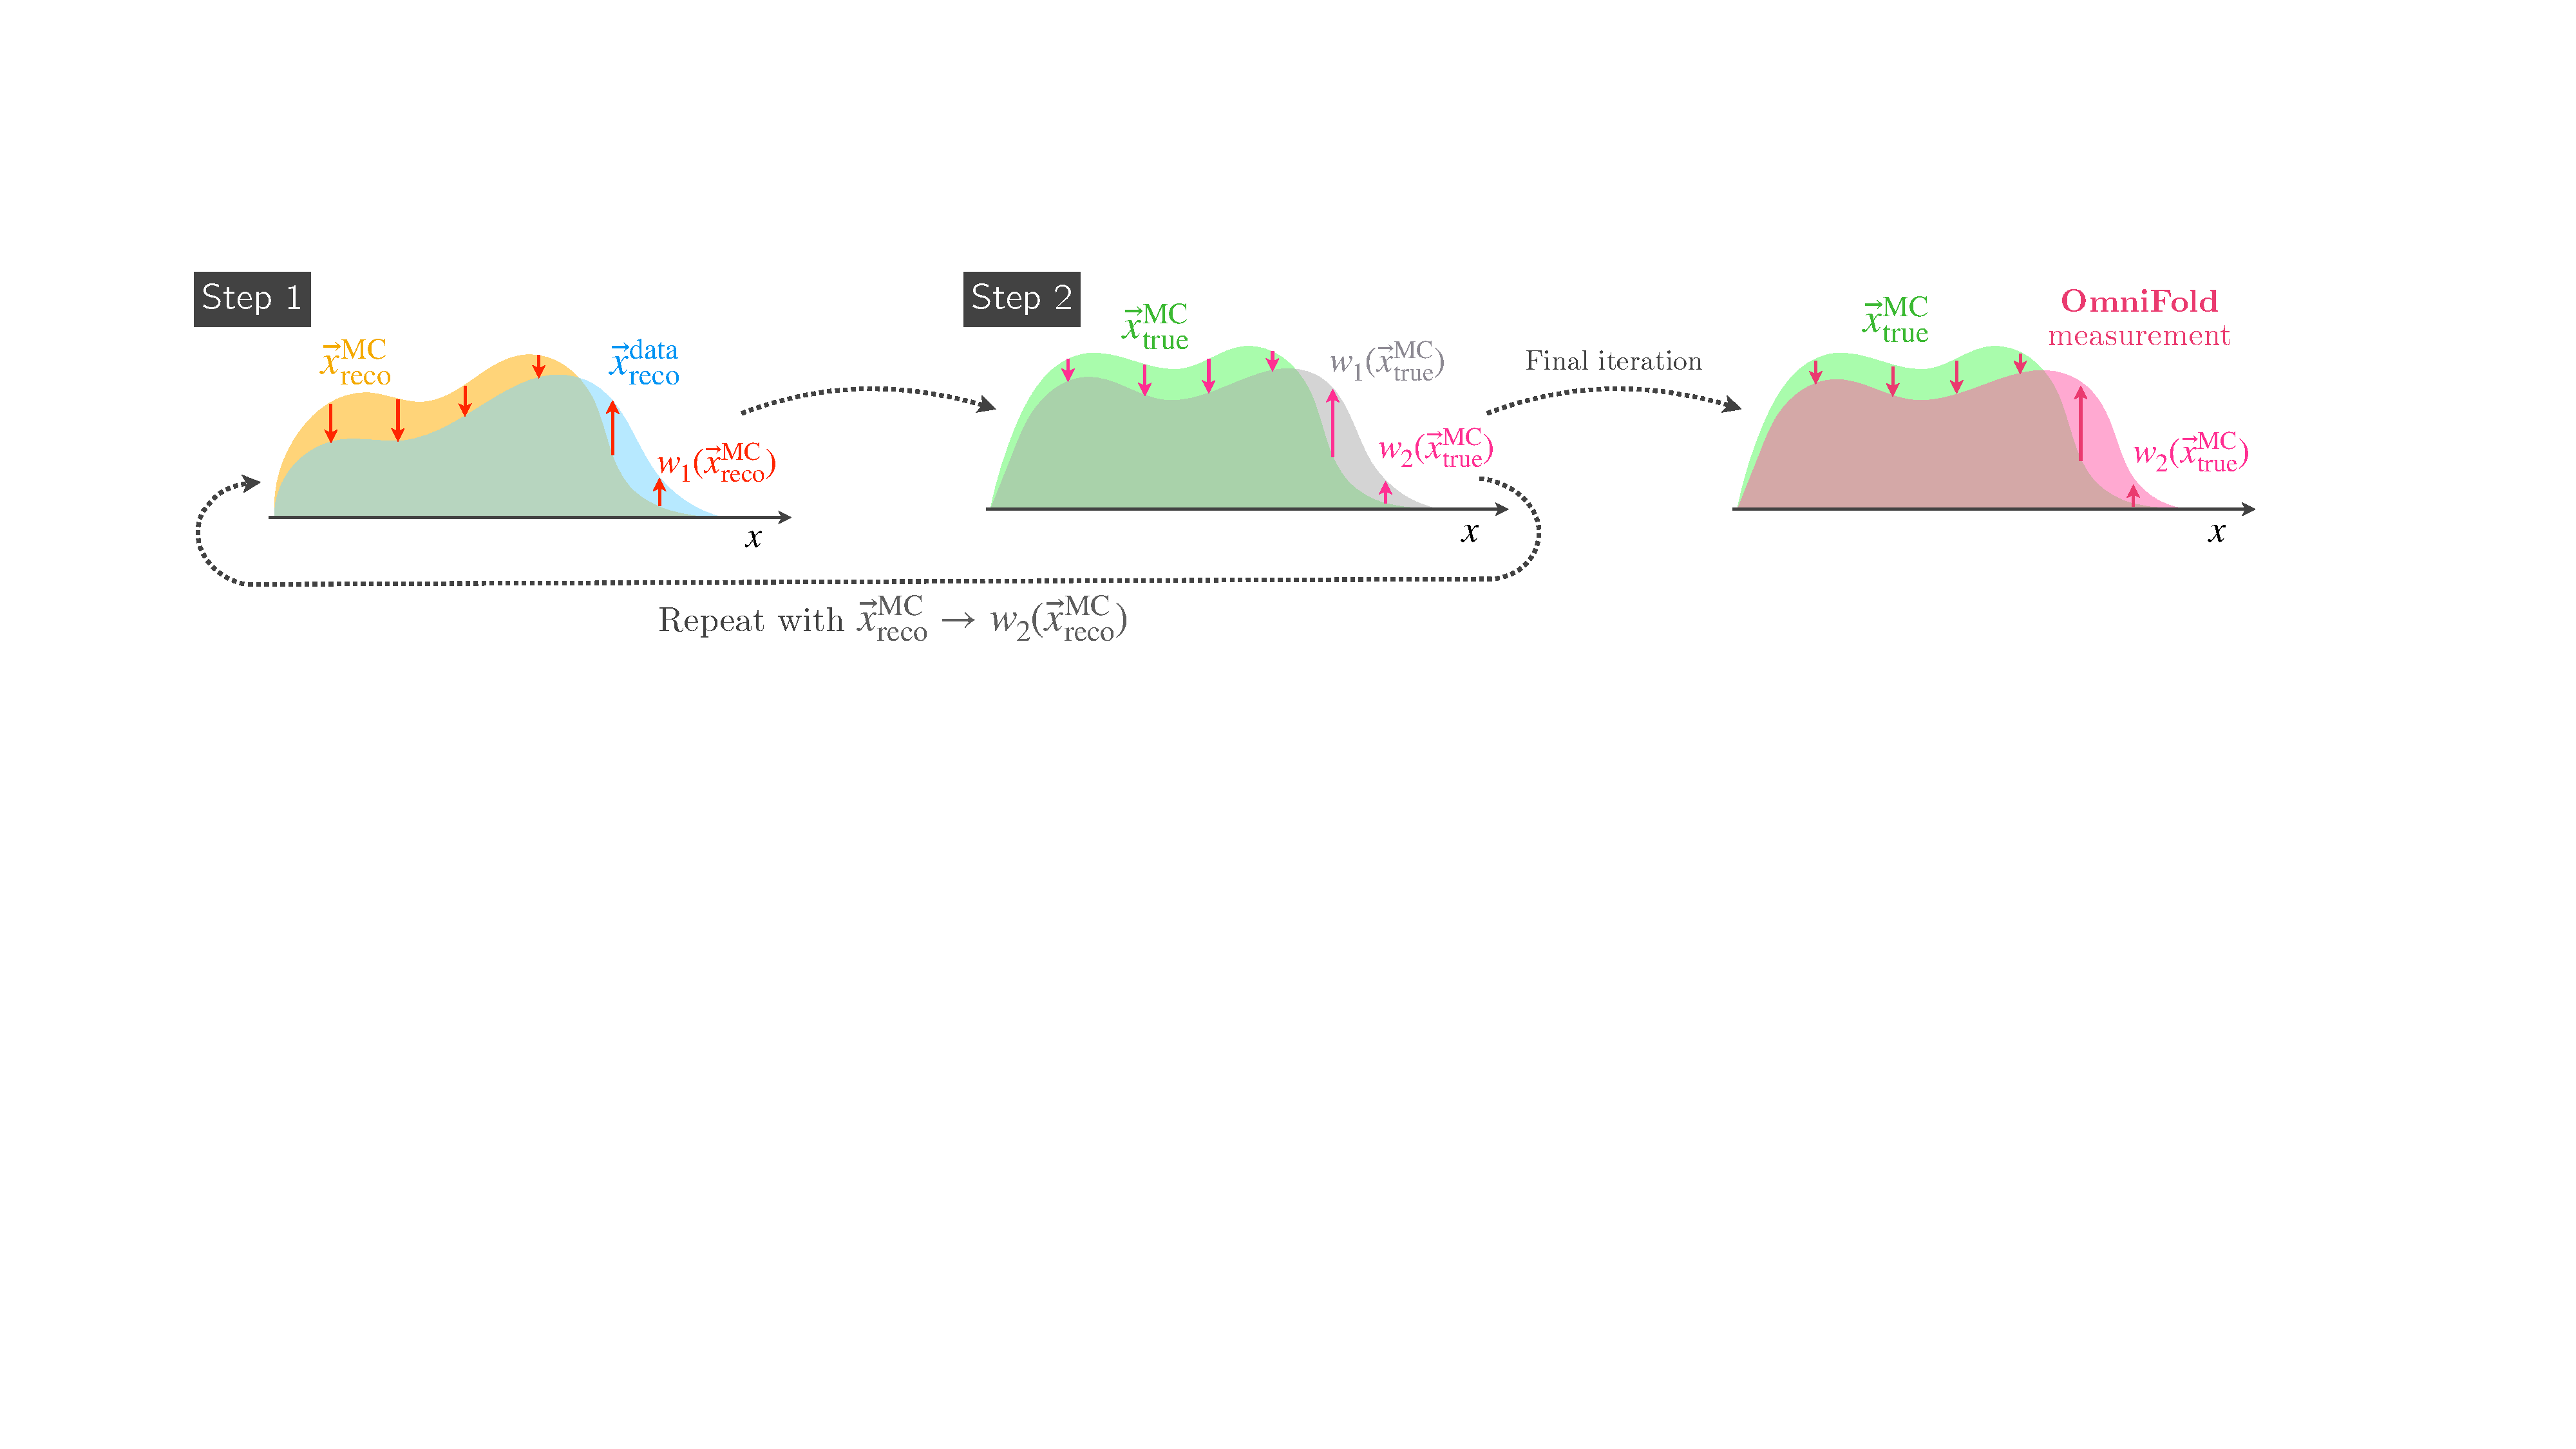
\includegraphics[width=1\linewidth]{figures/omnifold_fig_2025_04_24}
	\caption[Illustration of the OmniFold method]{Illustration of the OmniFold method. In Step 1, MC is corrected to match data at the detector level, producing a weighting function $w_1(\vec{x}_{\text{reco}}^{\text{ MC}})$. In Step 2, a new function $w_2(\vec{x}_{\text{true}}^{\text{ MC}})$ is learned based only on particle-level quantities. The method proceeds iteratively, refining the function $w_2(\vec{x}_{\text{true}}^{\text{ MC}})$ such that the particle-level MC can be reweighted to give event yields and kinematics that match those observed in the data~\cite{Canelli_2026}.}
	\label{fig:omnifold}
\end{figure}

One of the first unbinned approaches, OmniFold~\cite{PhysRevLett.124.182001} (Fig.~\ref{fig:omnifold}), uses classifiers to calculate the ratios \(\omega\) and \(\nu\). For \(i^\text{th}\) iteration, \(\omega_{i-1}(\mathbf{y})\) can be calculated using classifier \(f_\mathrm{meas., reco}\) which classifies a jet represented by \(\mathbf{y}\) as measured or reconstructed. Thus, 
\begin{equation}
	\omega_{i-1}(\mathbf{y}) = \frac{f_\mathrm{meas., reco}(\mathbf{y})}{1 - f_\mathrm{meas., reco}(\mathbf{y})}
\end{equation}
and \(\nu_{i-1}(\mathbf{y})\) can be calculated using classifier \(f_{i, i-1}\) which classifies a jet represented by \(\mathbf{x}\) as being generated from \(i^\text{th}\) or \((i-1)^\text{th}\) iteration. 
\begin{equation}
	\nu_{i-1}(\mathbf{x}) = \frac{f_{i, i-1}(\mathbf{x})}{1-f_{i, i-1}(\mathbf{x})}.
\end{equation}
Not every jet has a partner at the other level.
%
A generated jet whose reconstructed partner is lost, through the detector inefficiency, the resolution moving it out of the selection or a failed matching, is a \emph{miss}; a reconstructed jet without a generated partner, e.g.\ one formed from background fluctuations or moved into the selection by the resolution, is a \emph{fake}.
%
Misses have no \(\mathbf{y}\) and therefore no \(\omega_{i-1}(\mathbf{y})\), and fakes have no \(\mathbf{x}\) and therefore no \(\nu_{i-1}(\mathbf{x})\), so each needs its own estimate.
%
For misses, a classifier \(f^\mathrm{gen.}_{i, i-1}\) separates matched generated jets weighted by \(\omega_{i-1}(\mathbf{y})\) from those of the \((i-1)^\text{th}\) iteration; for fakes, a classifier \(f^\mathrm{reco.}_{i, i-1}\) separates matched reconstructed jets weighted by \(\nu_{i-1}(\mathbf{x})\) from those of the \((i-1)^\text{th}\) iteration,
\begin{equation}
	\omega_{i-1}(\mathbf{x}) = \frac{f^\mathrm{gen.}_{i, i-1}(\mathbf{x})}{1-f^\mathrm{gen.}_{i, i-1}(\mathbf{x})} ,
	\qquad
	\nu_{i-1}(\mathbf{y}) = \frac{f^\mathrm{reco.}_{i, i-1}(\mathbf{y})}{1-f^\mathrm{reco.}_{i, i-1}(\mathbf{y})} ,
\end{equation}
evaluated at the miss's \(\mathbf{x}\) and the fake's \(\mathbf{y}\) respectively. Thus, it takes 2-4 classifier trainings per unfolding iteration~\cite{andreassen2021scaffoldingsimulationsdeeplearning}.

The result of the unfolding is not a set of histograms but a weight for every generated jet.
%
Since each generated jet carries all the features \(\mathbf{x}\) it was unfolded with, any observable that is a function of \(\mathbf{x}\) can be computed from the weighted jets after the unfolding, in any binning, without repeating the unfolding: new observables can be studied with the same unfolded jets, as long as they are combinations of the unfolded features~\cite{PhysRevLett.124.182001,Canelli_2026}.
%
Observables that depend on information not contained in \(\mathbf{x}\) still require a new unfolding that includes it.
